\section{Theory}
	Compton scattering, as seen in \hyperref[th:1]{Figure 1}, is the scattering of photons by charged particles. The dispersed photon has less energy when the entering photon transfers some of its energy to the electron. has a lower frequency and a longer wavelength, per Planck's formula. Only the scattering angle for a specific target particle determines the wavelength shift in this type of scattering. According to the Compton formula, the wavelength shift increases with the scattering angle:

	\begin{equation}
		\lambda_{\theta}-\lambda_o = \frac{h}{m_ec}(1-cos\theta)
		\label{eq:1}
	\end{equation}

	Where, $\lambda_o$ is the incident wavelength of the photon, $\lambda_{\theta}$ is the scattered wavelength of the photon, h is Planck's constant,$m_e$ is the rest mass of the electron,c is the speed of light and $\theta$ is the scattering angle of the photon.

	\begin{figure}
		\centering
		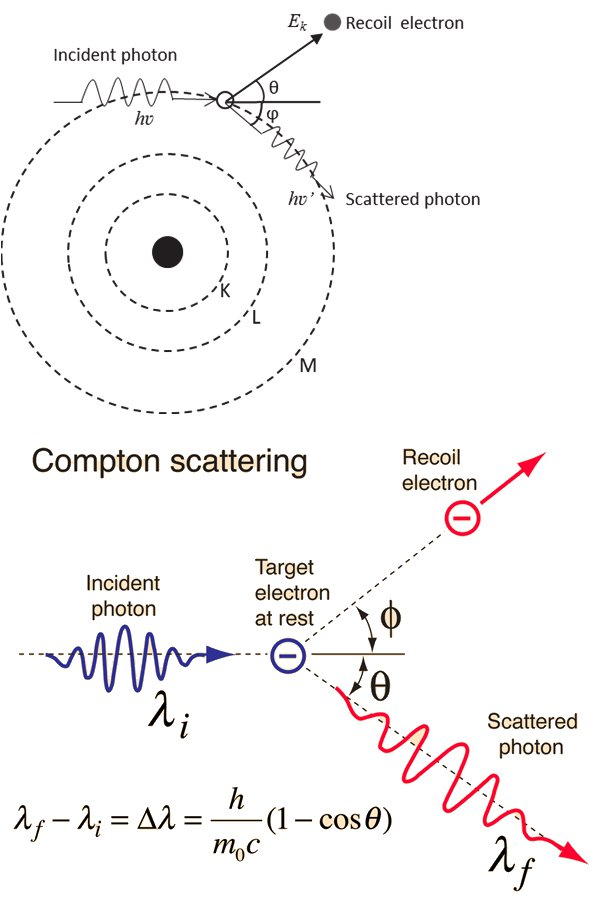
\includegraphics[width=0.6\columnwidth]{images/t1.png}
		\caption{Compton scattering}
		\label{th:1}
	\end{figure}

	The value $\frac{h}{m_ec} = 0.02426 \angstrom$ is called the Compton wavelength of the electron. In terms of energy, \hyperref[eq:1]{Equation 1} can be written as:

	\begin{equation}
		E_{\theta}=E_o\frac{1}{1+\gamma(1-cos\theta)}
		\label{eq:2}
	\end{equation}

	where $E_{\theta}$ and $E_o$ are energy of incident and scattered photons respectively and $\gamma=\frac{E_o}{m_ec^2}$. For high energy photons with ($\lambda\ll 0.02 \angstrom$ or $E \gg 511 keV$), the wavelength of the scattered radiation is always of the order of the Compton wavelength, whereas for low energy photons ($E \ll 511 keV$), the Compton shift is very small. In a nutshell, in a non-relativistic energy domain, the results of Compton scattering approach those anticipated by classical Thompson scattering. 

	Using quantum mechanical calculations, Klein-Nishina correctly formulated the differential Compton scattering cross-section formula. This equation is written as follows:

	\begin{equation}
		\begin{split}
			\frac{d\sigma}{d\Omega} = & r_o^2\frac{1+ cos^2\theta}{2(1+\gamma(1-cos\theta))^2} \times \\
		 & \left(1+\frac{\gamma^2(1-cos\theta)^2}{(1+ cos^2\theta)(1+\gamma(1-cos\theta))}\right)
		\end{split}
		\label{eq:3}
	\end{equation}

	where, $r_o=\frac{e}{4\pi\epsilon_om_ec^2} = 2.8179 \times 10^{-15}  $ is the classical electron radius.

	For dispersed photons, gamma rays from a $Cs^{137}$ source are used in this experiment. A calibrated scintillation detector set at varying scattering angles determines differences in incoming and scattered energy and wavelength of photons. By computing the calibration factor $C$ using the method below, the relative intensities $I\theta$ of the scattered radiation peaks may be compared with the predictions of the Klein-Nishina formula for the differential effective cross-section $\frac{d\sigma}{d\Omega}$. Thus:

	\begin{equation}
		C=\frac{1}{n}\sum_{\theta=0}^{n}\frac{I_\theta}{(\frac{d\sigma}{d\Omega})}
		\label{eq:4}
	\end{equation}
